  
\documentclass[letterpaper,aps,prc,superscriptaddress,nofootinbib,11pt,showpacs,floatfix]{revtex4-2}
\usepackage{graphicx}
\usepackage{comment}
\usepackage{setspace}
\usepackage{amsmath}
\usepackage{amssymb}
\usepackage{color}
\usepackage{indentfirst}
\usepackage{xspace}
\usepackage{hyperref}
\usepackage{verbatim}
\usepackage{epstopdf}
\usepackage{hyperref}
\usepackage{placeins}
\usepackage{xfrac}
\usepackage[table]{xcolor}
\usepackage{array}
\usepackage{changepage}
\usepackage{float}
\usepackage{enumitem}
\usepackage{listings}
\usepackage{listings}


\newcolumntype{P}[1]{>{\centering\arraybackslash}p{#1}}
\newcolumntype{M}[1]{>{\centering\arraybackslash}m{#1}}
\newcommand{\addmathvspace}{\vrule width 0pt height 4ex depth 2.5ex}
\newcommand{\sqs}{\mbox{$\sqrt{s}$}\xspace}
\newcommand{\ee}{\mbox{$e^{+} e^{-}$}\xspace}
\newcommand{\pp}{\mbox{$pp\,(p\bar{p})$ }\xspace}
\newcommand{\bfrac}[2]{\frac{\displaystyle #1}{\displaystyle #2}}
\newcommand{\ket}[1]{\left\vert #1\right\rangle}
\newcommand{\bra}[1]{\left\langle #1\right\vert}
\newcommand{\braket}[2]{\left\langle #1\vert #2\right\rangle}
\newcommand{\braketop}[3]{\left\langle #1\vert #2\vert #3\right\rangle}
\newcommand{\abs}[1]{\left\lvert #1\right\rvert}
\usepackage{chngcntr}
\counterwithin{figure}{section}

\numberwithin{equation}{section}
\lstset{
  basicstyle=\ttfamily,
  columns=fullflexible,
  frame=single,
  breaklines=true,
  postbreak=\mbox{\textcolor{red}{$\hookrightarrow$}\space},
}

\advance\day by -1


\bibliographystyle{ieeetr}


\setlength{\arrayrulewidth}{0.8mm}
\graphicspath{ {./Images/} }



\begin{document}

\title{Quantum Bitcoin and Cheque}
\author{Prasanta K. Panigrahi} 
\affiliation{Indian Institute of Science Education and Research, Kolkata, India}
\author{Ankan Mukherjee} 
\email{190260008@iitb.ac.in}
\affiliation{Indian Institute of Technology Bombay, Mumbai, India}
\author{Bikash Behera}




\tableofcontents
\newpage
\maketitle
\section*{Abstract}
The goal of the project is to explore the vulnerabilities of the current classical algorithm for encryption and hashing of crypto-currencies when subjected to quantum computing and to design more secure quantum algorithms. 
\section{Introduction}
We shall start with a background of the classical computations and then develop quantum methods for the same.
\subsection{Background}
Blockchain is the method used at present for secure peer to peer transactions through decentralized currencies\cite{btc}. It comprises peers broadcasting transactions on a decentralized ledger, secured by a digital signature. The signature can be generated uniquely by the use of a private key held by the node generating the signature only. The other peers can verify the authenticity of the signature using a widely available public key. Since copies of ledgers are possessed by all the peers on the network, it is imperative to develop a form of authenticity check on the ledgers. This is doing by using a special string called the nonce, which is in turn dependent on the contents of the ledger, to generate a hash satisfying some conditions. Mathematics show that brute force search is the only method for generating such a nonce. The probability of success is of the order of $\bfrac{1}{2^N}$, where $N$ is the number of bits used for hashing. For a standard 256-bit hash, the probability of finding a special nonce is too low for all practical purposes. Thus, "guessing" a nonce is nearly next to impossible at an individual level. To increase the security even further, blocks of transactions with a valid nonce are linked together in the form of a chain to prevent any fraudulent manipulation of previous transactions. This is called a block chain.
Quantum computing is a form of computing that uses the quantum mechanical states of particles, called qubits, to store information, instead of storing them on classical switches. Two special properties of qubits are that they can undergo superposition and entanglement. These properties allow special quantum algorithms to be developed, which speed an otherwise slow classical process. Quantum computers are speculated to posses serious threats to the classical computing algorithms\cite{enc_br}, including those used in the security of bitcoins. Quantum algorithms like Grover's algorithm and a more generalized version of it can search for the nonce much faster than a classical computer.
\subsection{Objectives}
The aim of the project is to find loopholes in the present system of cryptocurrency\cite{btc} when subjected to quantum computation and to find methods to improve the security. The problem at hand involves understanding the current methods of encryption and hashing, following by designing a quantum algorithm to break the same. At the last leg of the project, we shall solve these problems by using quantum algorithms for hashing.
\subsection{Applications}
Our work may be used to develop and enhance secure quantum algorithms for crypto-currencies. The algorithms presented in our work can also be used to design a new crypto-currency system on a real quantum computer back-end.
\subsection{System Requirements}
The code for our work uses Qiskit on a Jupyter Notebook on Python. The following are the minimum system requirements to run our code.\\
Processors: Intel Atom processor or Intel Core™ i3 processor or higher\\
Disk space: 1 GB or higher\\
Operating systems: Windows 7 or later, macOS 10.12.6 or later, and Ubuntu 16.04 or later\\
Python: 3.6 or higher\\
Numpy: 1.20.0 or higher\\
Jupyter Lab/Notebook: 6.3.0 or higher\\
Pip or Anaconda to install the above packages.\\
%The code is available \href{https://github.com/Ankan-Mukherjee/NIUS.git}{here}.
\newpage
\section{Blockchain}
In this section we shall discuss the main ideas of the blockchain system\cite{btc}. The basic unit of currency is defined as a block containing information about a transaction. The transaction is signed using an encrypted signature. The signature requires a private key to generate and a public key for verification. Details of some encryption methods are discussed later. %Direct to that section. 
Once a block signature has been verified, it is considered as a "legal block". To prevent peers from double spending, it is imperative to store all records of previous transactions in the block. This is made possible by storing some information of the previous block in the next block. Further, to ensure the correct chronology of these blocks, a timestamp (epoch) is used in the block, which marks the time of creation of the block. Since each block contains information about the previous block, the timestamp will be linear in the chain. Any discrepancies regarding this is indicative of a fraudulent block. Finally, we come to the main point that is relevant to our work. How does one ensure, in such a decentralized system, that there is no manipulation of information? This is achieved by hashing. Hashing the information in the block produces a 256-bit long hash. It is easy to verify a hash from a block but very difficult to generate a block that produces a given hash\cite{SHA}. Also, changing even a single character can cause a huge change in the hash. Details of hashing are discussed in more detail later %Direct to that section. 
Whether a block should be trusted or not is governed by the concept of "Proof of Work". This involves finding an arbitrary string, called the nonce, by brute-force, to be appended at the end of the block so that its hash starts with a certain minimum number of zeroes. To prevent manipulation of previous transactions, each block starts with the hash of the previous block. Resources in terms of CPU and electricity are used in huge quantities to generate these nonce. Any fraudulent party working individually to manipulate information in the blockchain will be unable to compete in terms of resources to find a proof of work for successive chains. This will in turn ensure that the longest chain is the most trusted one in case of a fork and the other short chains are automatically rejected. Figure \ref{Fig:1} shows the contents of a block. Figure \ref{Fig:2} shows a pictorial representation of a blockchain.\\

\begin{figure}[!htb]
   \begin{minipage}{0.25\textwidth}   
     \centering
     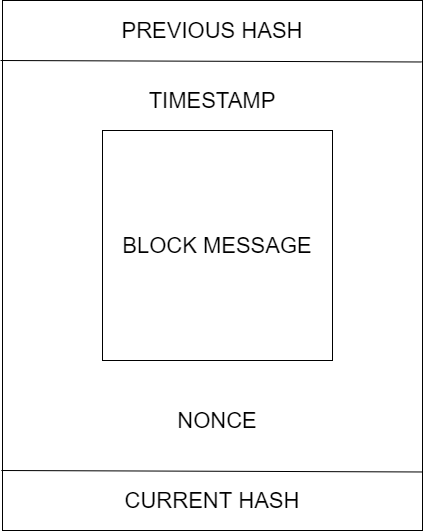
\includegraphics[width=1.1\linewidth]{fig1.png}
     \caption{A typical block}
     \label{Fig:1}
   \end{minipage}\hfill
   \begin{minipage}{0.65\textwidth}
     \centering
     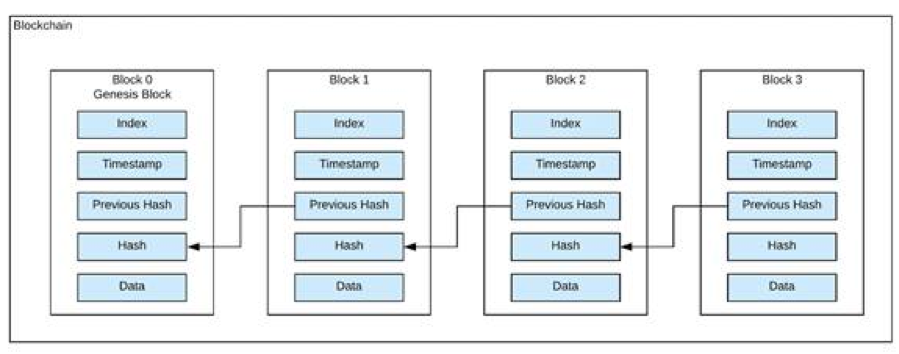
\includegraphics[width=1.1\linewidth]{fig2.png}
     \caption{The structure of a block chain\cite{bcpic}}
     \label{Fig:2}
   \end{minipage}\hfill
\end{figure}

The working of a blockchain system is summarized below.
\begin{enumerate}
\item New transactions are broadcast to all nodes.
\item Each node collects new transactions into a block.
\item Each node works on finding a difficult proof-of-work for its block.
\item When a node finds a proof-of-work, it broadcasts the block to all nodes.
\item Nodes accept the block only if all transactions in it are valid and not already spent.
\item Nodes express their acceptance of the block by working on creating the next block in the
chain, using the hash of the accepted block as the previous hash.
\end{enumerate}


\newpage
\section{Classical Algorithms}
In this section, we will take a look at each of the components of the blockchain implemented classically.
\subsection{Encryption}
Encryption is used to digitally sign transactions in a blockchain. Encryption is the process by which data is converted into a secure string of bits that can be uniquely decrypted. Encryption requires the use of a private key to decrypt an encrypted message and a public key to verify the encryption. Several encryption algorithms exists in the market, the most popular ones being the 3DES, AES and RSA\cite{enc_rsa}. 
\subsection{Hashing}
Hashing is the process by which a message of arbitrary lengths is converted to a bit string of fixed length. Unlike encryption, hashes are not unique. Several messages can have the same hash. Hashes must be easy to verify given a message. The reverse process, however, should be a hard one, i.e., given a hash, it should be practically impossible to find a message generating the hash. Hash collisions should also be rare, i.e., given a message and its hash, it should be practically impossible to find another message with the same hash. Finally, hashes must be distinctly different even for change of a single character in the message. Some commonly used hashing algorithms include SHA-1, Pearson Hash and SHA-256. In this paper, we will demonstrate the SHA-256. We will then design a surrogate hashing purpose that satisfies the aforementioned properties of hashes but is easy to simulate on a quantum computer.
\subsubsection*{SHA-256}
This comprises using XOR and shift operators on registers pre-loaded with existing values. The code for the same is mentioned below. The code is written in python.
\begin{lstlisting}
import math
import numpy as np

#The first 32 prime numbers are used to preset the hash registers by considering the fractional part of their square and cube roots
PRIMES=[2, 3, 5, 7, 11, 13, 17, 19, 23, 29, 31, 37, 41, 43, 47, 53, 59, 61, 67, 71, 73, 79, 83, 89, 97, 101, 103, 107, 109, 113, 127, 131, 137, 139, 149, 151, 157, 163, 167, 173, 179, 181, 191, 193, 197, 199, 211, 223, 227, 229, 233, 239, 241, 251, 257, 263, 269, 271,277,281,283,293,307,311]

#Right shift by n bits
def SHR_int(x,n):
    return x>>n
def SHR(s,n):
    x=int(s,2)
    return str(bin(x>>n))[2:].zfill(32)

#Right rotate by n bits
def ROTR_int(x,n):
    return (x>>n)|(x<<(32-n))&0xFFFFFFFF
def ROTR(s,n):
    x=int(s,2)
    return str(bin((x>>n)|(x<<(32-n))&0xFFFFFFFF))[2:].zfill(32)

#Linear combination in terms of XOR
def SIG0(x):
    return ROTR_int(x,2)^ROTR_int(x,13)^ROTR_int(x,22)
def SIG1(x):
    return ROTR_int(x,6)^ROTR_int(x,11)^ROTR_int(x,25)
    #return x
def sig0(s):
    x=int(s,2)
    return str(bin(ROTR_int(x,7)^ROTR_int(x,18)^SHR_int(x,3)))[2:].zfill(32)
def sig1(s):
    x=int(s,2)
    return str(bin(ROTR_int(x,17)^ROTR_int(x,19)^SHR_int(x,10)))[2:].zfill(32)
def che(x,y,z):
    return (x&y)|(~x&z)
def maj(x,y,z):
    return (x&y)^(y&z)^(z&x)

#Converts message to ASCII
def toAscii(message):
    return ''.join(str(bin(ord(c)))[2:].zfill(8) for c in message)

#Pads the message with zeroes till length is a multiple of 512 and then appends the length at the end
def padding(message_ascii):
    l=len(message_ascii)
    size=(l//512+1)*512
    pad=message_ascii+'1'
    for j in range(size-len(pad)-64):
        pad=pad+'0'
    pad=pad+str(bin(len(toAscii(message))))[2:].zfill(64)
    return pad,size

#Creates the message block
def message_block(message):
    padded_message=padding(toAscii(message))[0]
    nblocks=padding(toAscii(message))[1]//512
    w=[[None for _ in range(64)] for _ in range(nblocks)]
    for i in range(nblocks):
        for j in range(16):
            w[i][j]=padded_message[512*i+32*j:512*i+32*(j+1)]
        for j in range(16,64):
            w[i][j]=str(bin((int(sig1(w[i][j-2]),2)+int(w[i][j-7],2)+int(sig0(w[i][j-15]),2)+int(w[i][j-16],2))%int(2**32)))[2:].zfill(32)
    return w

#Compression where registers are continuously updated with values of the linear functions above to generate the hash
def compress(w,H0):
    H=H0
    for j in range(len(w)):
        wj=int(w[j],2)
        T1=(K[j]+wj+SIG1(H[4])+che(H[4],H[5],H[6])+H[7])%int(2**32)
        T2=(SIG0(H[0])+maj(H[0],H[1],H[2]))%int(2**32)  
        H=[(T1+T2)%int(2**32) ]+H[:-1]
        H[4]=(H[4]+T1)%int(2**32)
    return [(H0[i]+H[i])%int(2**32) for i in range(len(H))]

#Generates the hash in hexadecimal
def hashgen(message,H0):
    w=message_block(message)
    H=H0
    for i in range(len(w)):
        H=compress(w[i],H)
    return ''.join(str(hex(x))[2:].zfill(8) for x in H)

#Actually initializing the registers
K=[]
H=[]
for i in range(64):
    K.append(int(math.modf((PRIMES[i])**(1/3))[0]*(2**32)))
for i in range(8):
    H.append(int(math.modf((PRIMES[i])**(1/2))[0]*(2**32)))

#Inputiing the message from the user
message=input().rstrip()
#Printing the hash
print(hashgen(message,H))
\end{lstlisting}
Now we shall check the values of the hash for some sample strings. This can be done by running the code given above.\\
Message: \verb|Hello World|\\
Hash: \verb|a591a6d40bf420404a011733cfb7b190d62c65bf0bcda32b57b277d9ad9f146e|\\
Making a slight change\\
Message: \verb|Hello Workd|\\
Hash: \verb|5ab45e33f10c8c9eb8005ba117fbd6e9d4ce3e61d5b199c08cbb7bbebf58cf68|\\
We see that the hash changes significantly.
\subsubsection*{Surrogate Hash Function: Pearson Hashes and LFSRs}
The SHA-256 is a rather cumbersome method of hashing that requires significant amount of time and memory when simulating using qiskit. To overcome this difficulty, we will use a surrogate hash called the Pearson Hash\cite{pearson}. The Pearson Hash makes use of a lookup table, which can be achieved using Linear Feedback Shift Registers (LFSR)\cite{lfsr}. These are easy to implement in qiskit\cite{qlfsr}, and the hash so generated satisfies the properties of a good hash. Since the purpose of our project is the search for nonce for a given hashing algorithm and not hashing, using a surrogate hashing algorithm will make no difference.

An LFSR comprises shift registers in which, at each iteration, the elements shift to the adjacent register (like in an ordinary shift register) and the first register takes the value of a linear function of some of the registers. Galois Theory of Fields dictates the working of these LFSRs. The values which are XORed are called taps. %See Appendix
The LFSR structure is shown in Figure \ref{Fig:3}
where $\oplus$ denotes XOR.
\begin{figure}[!htb]
   \begin{minipage}{\textwidth}
     \centering
     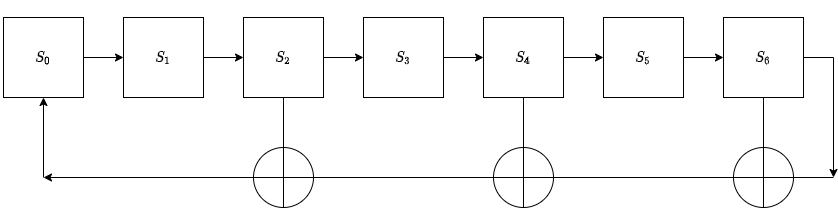
\includegraphics[width=1\linewidth]{fig3.png}
     \caption{A sample LFSR with taps at 2,4 and 6}
     \label{Fig:3}
   \end{minipage}
\end{figure}

Pearson hashing uses two LFSRs. It works by taking the XOR of a character with the register and then performing two different sets of LFSRs. While LFSRs by themselves are reversible, it is impossible to extract the characters of a message from the hashing owing to the repeated XOR operations.
\subsection{The Epoch, Nonce and Mining}
The time stamp appended in a block (see \ref{Fig:1}) is called an epoch. It is a 4-byte integer that represents the number of seconds passed from January 1, 1970 00:00 UTC.\\
The nonce is the arbitrary string that needs to be found by brute force algorithms to ensure the hash starts with a certain minimum number of zeroes. The process of finding the nonce is called "mining" in the language of crypto-currencies. Mining requires heavy use of resources like electricity and computing power. Bitcoin miners are often provided with incentives for the process. Since we have a 256-bit hash, mining success probability is of the order of $2^{-256}$, a number that is astronomically small. Mining is a form of proof of work that ensures fraudulent individuals do not take advantage of a decentralized ledger. If the majority mines honest blocks, it becomes easy for someone or the other to get the nonce. In case of a fork in terms of two different blockchains with appropriate nonces, the longer blockchain gets accepted.\\
The hash function that we are using generates 8-bit long hashes. Our nonce can thus be 8-bit long, which can be represented by a single character.
\newpage
\section{Quantum Computing Foundations}
\noindent Before delving into quantum algorithms, it would be worthwhile to take a quick glance into the basics of quantum computing. Quantum computing uses the quantum state of a particle as the building block of information. Each such particle is called a qubit. These qubits follow the postulates of quantum mechanics\cite{shankar}, namely
\begin{enumerate}
\item The state of the particle is represented as a vector $\ket{\psi(t)}$ in a Hilbert Space.
\item The independent variables $x$ and $p$ of classical mechanics are represented by Hermitian operators $X$ and $P$ satisfying $\braketop{x}{X}{x\prime}=x\delta(x-x\prime)$ and $\braketop{x}{P}{x\prime}=-\iota\hbar\delta\prime(x-x\prime)$.
\item If a particle is in a state $\ket{\psi}$, measurement of the variable corresponding to the operator $\Omega$ will yield one of the eigenvalues $\omega$ with probability $P(\omega)\propto\left\lvert\braket{\omega}{\psi}\right\rvert ^2$. The state of the system will change from $\ket{\psi}$ to $\ket{\omega}$ as a result of the measurement.
\item The state vector $\ket{\psi}$ obeys the Schrödinger Equation $\iota\hbar\bfrac{d}{dt}\ket{\psi(t)}=\hat{H}\ket{\psi(t)}$, where $\hat{H}$ is the quantum Hamiltonian operator.
\end{enumerate}
\subsection{Qubits}
As discussed before, qubits are the particles whose quantum states store the necessary information. To retrieve the information, we perform measurements using an unitary operator that has $2$ eigenstates. These eigenstates are denoted as $\ket{0}$ and $\ket{1}$. Since the measurement operator is unitary, these eigenstates are orthonormal. The $2$ eigenstates represents the two possible values of a classical bit, except that quantum mechanics allows \textbf{superposition} and \textbf{entanglement}, which are discussed subsequently.
\subsection{Superposition}
In general, quantum mechanics is probabilistic and not deterministic, i.e., the two eigenstates may not be the only possible states of a qubit. A qubit can be in a superposition of two states, in the form $\ket{\psi}=\bfrac{\alpha\ket{0}+\beta\ket{1}}{\sqrt{2}}$ with the only requirement that $\abs{\alpha}^2+\abs{\beta}^2=1$ (this is called normalization. When a measurement is performed on this state, the state collapses to either $\ket{0}$ with probability $\abs{\alpha}^2$ or to $\ket{1}$ with probability $\abs{\beta}^2$.\\
Since $\ket{0}$ and $\ket{1}$ are orthonormal, they form an orthonormal basis for the states. Each state can then be represented in the form of a vector as
\begin{equation}
\label{eq:4.1}
\ket{\psi}=\bfrac{\alpha\ket{0}+\beta\ket{1}}{\sqrt{2}}=
\begin{pmatrix}
\alpha\\
\beta
\end{pmatrix}
\end{equation}
This immediately yields
\begin{equation*}
\ket{0}=
\begin{pmatrix}
1\\
0
\end{pmatrix}\quad
\ket{1}=
\begin{pmatrix}
0\\
1
\end{pmatrix}
\end{equation*}
Any state can now be written as the linear combination of these two states. Upon measurement, however, the superposition is lost and the system collapses to either of the eigenstates.\\
Since an operator operates on one state to produce another state, they can be viewed as transforming one vector to another. Thus, they can be expressed as matrices. The postulates of quantum mechanics dictate that these operators must be unitary to yield compatible, real-valued measurement.
\subsection{Multiple Qubits}
Often we encounter multiple qubit systems. The state of such a system is decided by the states of the individual qubits. The direct product of the basis states form the basis (also called pure states) for the multi-qubit system.\\
As an example, consider the $2$-qubit system. The basis set for such a system will be formed by the $4$ basis states : $\ket{0}\otimes\ket{0}$, $\ket{0}\otimes\ket{1}$, $\ket{1}\otimes\ket{0}$ and $\ket{1}\otimes\ket{1}$. These are notationally written as \\
\begin{equation*}
\begin{split}
\ket{00}&=
\begin{pmatrix}
1\\
0
\end{pmatrix}
\otimes
\begin{pmatrix}
1\\
0
\end{pmatrix}=
\begin{pmatrix}
1\\
0\\
0\\
0
\end{pmatrix}
\\
\ket{01}&=
\begin{pmatrix}
1\\
0
\end{pmatrix}
\otimes
\begin{pmatrix}
0\\
1
\end{pmatrix}=
\begin{pmatrix}
0\\
1\\
0\\
0
\end{pmatrix}
\end{split}
\end{equation*}
\begin{equation*}
\begin{split}
\ket{10}&=
\begin{pmatrix}
0\\
1
\end{pmatrix}
\otimes
\begin{pmatrix}
1\\
0
\end{pmatrix}=
\begin{pmatrix}
0\\
0\\
1\\
0
\end{pmatrix}
\\
\ket{11}&=
\begin{pmatrix}
0\\
1
\end{pmatrix}
\otimes
\begin{pmatrix}
0\\
1
\end{pmatrix}=
\begin{pmatrix}
0\\
0\\
0\\
1
\end{pmatrix}
\end{split}
\end{equation*}

Any two-qubit system is a superposition of the $4$ states mentioned above. However, not all two-qubit states are expressible as a direct product of two one-qubit states. This is called \textbf{entanglement}, which forms the basis for quantum teleportation, and spooky action at a distance.\\
For a multi-qubit system, we often use the decimal equivalent of a binary number to express the basis. For example, in a 4-qubit system, $\ket{12}=\ket{1100}=\ket{1}\otimes\ket{1}\otimes\ket{0}\otimes\ket{0}$.

\subsection{Quantum Gates}
Any logical circuit requires the use of gates. A classical circuit uses AND, NOT, OR etc. as gates. Likewise, a quantum circuit uses unitary operators as gates. A gate can be expressed as a matrix. Some of the useful gates are presented below.

\subsubsection*{Hadamard Gate}
The Hadamard gate is a \textbf{one-qubit} gate that is denoted by $H$. It performs the operation of transforming the standard basis of $\ket{0}$ and $\ket{1}$ into the Hadamard basis of $\ket{+}$ and $\ket{-}$ respectively as follows.
\begin{equation*}
\begin{split}
H\ket{0}&=\ket{+}=\bfrac{\ket{0}+\ket{1}}{\sqrt{2}}=
\bfrac{1}{\sqrt{2}}
\begin{pmatrix}
1\\
1
\end{pmatrix}\\
H\ket{1}&=\ket{-}=\bfrac{\ket{0}-\ket{1}}{\sqrt{2}}=
\bfrac{1}{\sqrt{2}}
\begin{pmatrix}
1\\
-1
\end{pmatrix}\\
\end{split}
\end{equation*}
The matrix representation is
\begin{equation*}
H=
\begin{pmatrix}
1&1\\
1&-1
\end{pmatrix}
\end{equation*}
The corresponding circuit diagram is given in figure \ref{Fig:4.1}
\begin{figure}[!htb]
   \begin{minipage}{\textwidth}
     \centering
     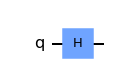
\includegraphics[scale=1]{fig04.01.png}
     \caption{Hadamard gate}
     \label{Fig:4.1}
   \end{minipage}
\end{figure}



\subsubsection*{X Gate}
The Pauli-$X$ gate is a \textbf{one-qubit} gate that is denoted by $X$. It performs the operation of a classical NOT, i.e., it operates like the Pauli matrix $\sigma_x$ as follows.
\begin{equation*}
\begin{split}
X\ket{0}&=\ket{1}=
\begin{pmatrix}
0\\
1
\end{pmatrix}\\
X\ket{1}&=\ket{0}=
\begin{pmatrix}
1\\
0
\end{pmatrix}\\
\end{split}
\end{equation*}
The matrix representation is
\begin{equation*}
X=
\begin{pmatrix}
0&1\\
1&0
\end{pmatrix}
\end{equation*}
The corresponding circuit diagram is given in figure \ref{Fig:4.2}
\begin{figure}[!htb]
   \begin{minipage}{\textwidth}
     \centering
     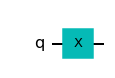
\includegraphics[scale=1]{fig04.02.png}
     \caption{$X$ gate}
     \label{Fig:4.2}
   \end{minipage}
\end{figure}

\subsubsection*{Y Gate}
The Pauli-$Y$ gate is a \textbf{one-qubit} gate that is denoted by $Y$. It operates like the Pauli matrix $\sigma_y$ as follows.
\begin{equation*}
\begin{split}
Y\ket{0}&=-\iota\ket{1}=
\begin{pmatrix}
0\\
-\iota
\end{pmatrix}\\
Y\ket{1}&=\iota\ket{0}=
\begin{pmatrix}
\iota\\
0
\end{pmatrix}\\
\end{split}
\end{equation*}
The matrix representation is
\begin{equation*}
Y=
\begin{pmatrix}
0&-\iota\\
\iota&0
\end{pmatrix}
\end{equation*}
The corresponding circuit diagram is given in figure \ref{Fig:4.3}
\begin{figure}[!htb]
   \begin{minipage}{\textwidth}
     \centering
     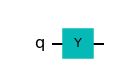
\includegraphics[scale=1]{fig04.03.png}
     \caption{$Y$ gate}
     \label{Fig:4.3}
   \end{minipage}
\end{figure}

\subsubsection*{Z Gate}
The Pauli-$Z$ gate is a \textbf{one-qubit} gate that is denoted by $Z$. It operates like the Pauli matrix $\sigma_z$ as follows.
\begin{equation*}
\begin{split}
Z\ket{0}&=\ket{0}=
\begin{pmatrix}
1\\
0
\end{pmatrix}\\
Z\ket{1}&=-\ket{1}=
-\begin{pmatrix}
0\\
1
\end{pmatrix}\\
\end{split}
\end{equation*}
The matrix representation is
\begin{equation*}
Z=
\begin{pmatrix}
1&0\\
0&-1
\end{pmatrix}
\end{equation*}
The corresponding circuit diagram is given in figure \ref{Fig:4.4}
\begin{figure}[!htb]
   \begin{minipage}{\textwidth}
     \centering
     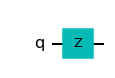
\includegraphics[scale=1]{fig04.04.png}
     \caption{$Z$ gate}
     \label{Fig:4.4}
   \end{minipage}
\end{figure}

\subsubsection*{$R_x$ Gate}
The $R_x$ gate is a \textbf{one-qubit} unitary gate that takes a parameter $\theta$. It is given by the matrix 
\begin{equation*}
R_x(\theta)=
\begin{pmatrix}
\cos\left(\bfrac{\theta}{2}\right)&-\iota \sin\left(\bfrac{\theta}{2}\right)\\
-\iota \sin\left(\bfrac{\theta}{2}\right)&\cos\left(\bfrac{\theta}{2}\right)
\end{pmatrix}
\end{equation*}

\subsubsection*{$R_y$ Gate}
The $R_y$ gate is a \textbf{one-qubit} unitary gate that takes a parameter $\theta$. It is given by the matrix 
\begin{equation*}
R_y(\theta)=
\begin{pmatrix}
\cos\left(\bfrac{\theta}{2}\right)&\sin\left(\bfrac{\theta}{2}\right)\\
\sin\left(\bfrac{\theta}{2}\right)&\cos\left(\bfrac{\theta}{2}\right)
\end{pmatrix}
\end{equation*}

\subsubsection*{$R_z$ Gate}
The $R_z$ gate is a \textbf{one-qubit} unitary gate that takes a parameter $\theta$. It is given by the matrix 
\begin{equation*}
R_z(\theta)=
\begin{pmatrix}
e^{-\iota\frac{\theta}{2}}&0\\
0&e^{\iota\frac{\theta}{2}}
\end{pmatrix}
\end{equation*}

\subsubsection*{CX Gate}
The CNOT (or CX) gate is a \textbf{two-qubit} gate that is denoted by $CX$. It operates a classical NOT, i.e., an $X$ gate on the second qubit if the first qubit is $\ket{1}$. Its working is shown below.
\begin{equation*}
\begin{split}
CX\ket{00}&=\ket{00}=
\begin{pmatrix}
1\\
0\\
0\\
0
\end{pmatrix}\\
CX\ket{01}&=\ket{01}=
\begin{pmatrix}
0\\
1\\
0\\
0
\end{pmatrix}\\
CX\ket{10}&=\ket{11}=
\begin{pmatrix}
0\\
0\\
0\\
1
\end{pmatrix}\\
CX\ket{11}&=\ket{10}=
\begin{pmatrix}
0\\
0\\
1\\
0
\end{pmatrix}\\
\end{split}
\end{equation*}
The matrix representation is
\begin{equation*}
CX=
\begin{pmatrix}
1&0&0&0\\
0&1&0&0\\
0&0&0&1\\
0&0&1&0
\end{pmatrix}
\end{equation*}
Note that the order of the qubits is important here. The corresponding circuit diagram is given in figure \ref{Fig:4.5}
\begin{figure}[!htb]
   \begin{minipage}{\textwidth}
     \centering
     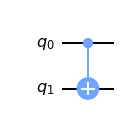
\includegraphics[scale=1]{fig04.05.png}
     \caption{$CX$ gate}
     \label{Fig:4.5}
   \end{minipage}
\end{figure}

\subsubsection*{CZ Gate}
The CZ gate is a \textbf{two-qubit} gate that is denoted by $CZ$. It is like a classical AND gate which flips the sign if and only if both qubits are $\ket{1}$. Its working is shown below.
\begin{equation*}
\begin{split}
CZ\ket{00}&=\ket{00}=
\begin{pmatrix}
1\\
0\\
0\\
0
\end{pmatrix}\\
CZ\ket{01}&=\ket{01}=
\begin{pmatrix}
0\\
1\\
0\\
0
\end{pmatrix}
\end{split}
\end{equation*}
\begin{equation*}
\begin{split}
CZ\ket{10}&=\ket{10}=
\begin{pmatrix}
0\\
0\\
1\\
0
\end{pmatrix}\\
CZ\ket{11}&=-\ket{11}=
-\begin{pmatrix}
0\\
0\\
0\\
1
\end{pmatrix}\\
\end{split}
\end{equation*}
The matrix representation is
\begin{equation*}
CZ=
\begin{pmatrix}
1&0&0&0\\
0&1&0&0\\
0&0&1&0\\
0&0&0&-1
\end{pmatrix}
\end{equation*}
Note that the order of the qubits is unimportant here. The corresponding circuit diagram is given in figure \ref{Fig:4.6}
\begin{figure}[!htb]
   \begin{minipage}{\textwidth}
     \centering
     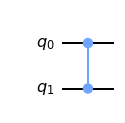
\includegraphics[scale=1]{fig04.06.png}
     \caption{$CZ$ gate}
     \label{Fig:4.6}
   \end{minipage}
\end{figure}

\subsubsection*{SWAP Gate}
The SWAP gate is a \textbf{two-qubit} gate that is denoted by $SWAP$. It swaps the two qubits. Its working is shown below.
\begin{equation*}
\begin{split}
CX\ket{00}&=\ket{00}=
\begin{pmatrix}
1\\
0\\
0\\
0
\end{pmatrix}\\
CX\ket{01}&=\ket{10}=
\begin{pmatrix}
0\\
0\\
1\\
0
\end{pmatrix}
\end{split}
\end{equation*}
\begin{equation*}
\begin{split}
CX\ket{10}&=\ket{01}=
\begin{pmatrix}
0\\
1\\
0\\
0
\end{pmatrix}\\
CX\ket{11}&=\ket{11}=
\begin{pmatrix}
0\\
0\\
0\\
1
\end{pmatrix}\\
\end{split}
\end{equation*}
The matrix representation is
\begin{equation*}
SWAP=
\begin{pmatrix}
1&0&0&0\\
0&0&1&0\\
0&1&0&0\\
0&0&0&1
\end{pmatrix}
\end{equation*}
Note that the order of the qubits is unimportant here. The corresponding circuit diagram is given in figure \ref{Fig:4.7}
\begin{figure}[!htb]
   \begin{minipage}{\textwidth}
     \centering
     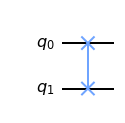
\includegraphics[scale=1]{fig04.07.png}
     \caption{$SWAP$ gate}
     \label{Fig:4.7}
   \end{minipage}
\end{figure}

\subsubsection*{MCT Gate}
The Multi Controlled Toffoli (MCT) gate is a \textbf{multi-qubit} gate that is denoted by $MCT$.It puts a negative sign on the target qubit if all the control qubits are $\ket{1}$.
The matrix representation is
\begin{equation*}
MCT=
\begin{pmatrix}
1&0&\dots&0&0\\
0&1&\dots&0&0\\
\vdots&\vdots&\ddots&\vdots&\vdots\\
0&0&\dots&1&0\\
0&0&\dots&0&-1
\end{pmatrix}
\end{equation*}
Note that the order of the qubits is unimportant here. The corresponding circuit diagram is given in figure \ref{Fig:4.8}
\begin{figure}[!htb]
   \begin{minipage}{\textwidth}
     \centering
     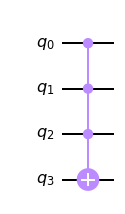
\includegraphics[scale=1]{fig04.08.png}
     \caption{$MCT$ gate on $4$ qubits}
     \label{Fig:4.8}
   \end{minipage}
\end{figure}


Note that gates can be cascaded. The order of operations of the gates is important. If we have gates $G_1$ and $G_2$, then $G_1G_2\ket{\psi}$ means $G_2$ is operated first on $\ket{\psi}$ and then $G_1$ is applied on the resulting states. Sometimes, cascading gates may result in an equivalent gate. As an example, cascading the operation of $H$ followed by $X$ is same as $R_y$ since $XH=R_y$ (this is trivial and can be easily verified). 

\subsection{Entanglement}
Entanglement is the is phenomenon where two or more quantum particles (qubits) are correlated and measurement of one particle collapses the wavefunction of the other particles. A simple example of an entangled state is
\begin{equation*}
\ket{\psi}=\bfrac{\ket{00}+\ket{11}}{\sqrt{2}}
\end{equation*}
If the measurement of the first particle collapses to $\ket{0}$, the second particle collapses to $\ket{0}$ as well.\\
Note that entangled states cannot be factored into a direct product of two single qubit states. This is a phenomenon that is purely quantum mechanical and is extremely useful in secure communication. This is because, since a measurement of any one particle collapses the wavefunction of the other particles as well, eavsdroppers will never go unnoticed, unlike in the classical case. To measure entanglement, we use the concepts of Bell's inequality. Entanglement has led to several paradoxes as well, the most famous of which is the EPR paradox.%This is presented in appendix
\newpage
\section{Grover's Algorithm}
Grover's search algorithm\cite{grover} is an important quantum algorithm that provides an edge over all classical algorithms in database search. Grover's algorithm shall form the backbone for our search for the nonce. The algorithm uses repeated iterations of a quantum oracle (an oracle stands for a special function) and a diffuser on a superposition of $\ket{0}$ and $\ket{1}$.
\subsection{Oracle}
The oracle is the function that "marks" the states which are the successful search results by applying a negative sign on it. Consider the state $\ket{\omega}$ to be successful. Denote the oracle by $U_\omega$ so that
\begin{equation}
\label{eq:5.1}
U_\omega\ket{x}=
\begin{cases}
\ket{x}&x\neq\omega\\
-\ket{x}&x=\omega
\end{cases}
\end{equation}
The purpose of the oracle is to reflect the coefficient of "solution state ket" about 0, keeping the other coefficients intact. This will help the diffuser amplify amplitudes.
\subsection{Diffuser}
The diffuser is the key component of the Grover Search algorithm. The diffuser amplifies the amplitude of the solution states. It does this by reflecting the amplitudes of the states about the average amplitude. We denote the diffuser by $U_s$, so that
\begin{equation}
\label{eq:5.2}
U_s=2\ket{s}\bra{s}-\mathbb{I}
\end{equation}
where $\ket{s}$ is some arbitrary state.
This is indeed a reflection about the state $\ket{s}$. This is because any arbitrary state $\ket{\psi}$ can be written as $\ket{\psi}=\cos\alpha\ket{s}+\sin\alpha\ket{s_\perp}$ where $\ket{s_\perp}$ is orthogonal to $\ket{s}$. Then we have
\begin{equation}
\label{eq:5.3}
\begin{split}
U_s\ket{\psi}&=U_s\left(\cos\alpha\ket{s}+\sin\alpha\ket{s_\perp}\right)\\
&=\left(2\ket{s}\bra{s}-\mathbb{I}\right)\left(\cos\alpha\ket{s}+\sin\alpha\ket{s_\perp}\right)\\
&=\cos\alpha\left(2\ket{s}\bra{s}\ket{s}-\ket{s}\right)+\sin\alpha\left(2\ket{s_\perp}\bra{s_\perp}\ket{s_\perp}-\ket{s_\perp}\right)\\
&=\cos\alpha\left(2\ket{s}-\ket{s}\right)+\sin\alpha\left(-\ket{s_\perp}\right)\\
&=\cos\alpha\ket{s}-\sin\alpha\ket{s_\perp}
\end{split}
\end{equation}
and we can clearly see that this is a reflection about the $\ket{s}$ axis.


Note that we can write $\ket{s}$ as a sum of two components, one linear function of $\ket{\omega}$ and the other a linear function of a state $\ket{s\prime}$ orthogonal to $\ket{\omega}$. Thus
\begin{equation}
\label{eq:5.4}
\ket{s}=\sin\theta\ket{\omega}+\cos\theta\ket{s\prime}
\end{equation}
Each iteration will comprise $U_s U_{\omega}$, i.e., reflection of $\ket{s}$ about $\ket{s\prime}$ followed by reflection about $\ket{s}$. This results in amplitude amplification. 

\subsection{The Method}
\noindent The method of applying Grover's Search is quite simple.
\begin{enumerate}
\item Initialize $\ket{s}=\bfrac{\ket{0}+\ket{1}}{2}$.
\item Perform $U_{\omega}$ on the state to reflect component along $\ket{\omega}$, keeping components orthogonal to $\ket{\omega}$ intact.
\item Apply $U_{s}$ on this state to reflect the state about $\ket{s}$
\item Repeat steps $2$ and $3$ till search is complete.
\end{enumerate}
The above steps are illustrated in %figure.\\
Now will we actually implement the oracle and the diffuser using quantum logic gates. First let us take a look at the oracle.
\subsubsection*{Implementation of the Oracle}
The oracle is implemented using a phase kickback mechanism. Consider the CNOT gate in \ref{Fig:5.1}. The CNOT gate acts as shown below.
\begin{equation}
\label{eq:5.5}
\begin{split}
&CX\ket{00}=\ket{00}\\
&CX\ket{01}=\ket{01}\\
&CX\ket{10}=\ket{11}\\
&CX\ket{11}=\ket{10}\\
\end{split}
\end{equation}
\begin{figure}[!htb]
   \begin{minipage}{\textwidth}
     \centering
     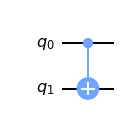
\includegraphics[scale=1]{fig05.01.png}
     \caption{CNOT gate}
     \label{Fig:5.1}
   \end{minipage}
\end{figure}

Now, if we have our classical function $f$ behaving as 
\begin{equation}
\label{eq:5.6}
\begin{split}
f(\omega)&=1\\
f(s)&=0\quad\forall s\neq\omega
\end{split}
\end{equation}
Then we can set up an output qubit as
$$
\ket{out}=\ket{-}=\bfrac{\ket{0}+\ket{1}}{\sqrt{2}}
$$
so that
\begin{equation}
\label{eq:5.7}
CX\ket{f(x)\ out}=
\begin{cases}
\ket{f(x)\ out}&f(x)=0\\
-\ket{f(x)\ out}&f(x)=1
\end{cases}
\end{equation}
Thus we get our oracle. The oracle circuit is shown in \ref{Fig:5.2}. 
\begin{figure}[!htb]
   \begin{minipage}{\textwidth}
     \centering
     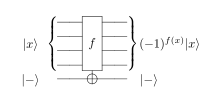
\includegraphics[scale=1]{fig05.02.png}
     \caption{The Oracle}
     \label{Fig:5.2}
   \end{minipage}
\end{figure}

\subsubsection*{Implementation of the Diffuser}
The diffuser has the equation as per equation \ref{eq:5.3}. To implement the diffuser on the state $\ket{000\cdots0}$, we just need to flip all qubits using $X$ gates and then apply a multi-controlled $Z$-gate. Since we are starting with the state $\ket{+++\cdots+}$, we need to apply a $H$-gate in the beginning and at the end to got to $\ket{000\cdots0}$ and revert back. Figure \ref{Fig:5.3} shows the diffuser circuit for 8 qubits.
\begin{figure}[!htb]
   \begin{minipage}{\textwidth}
     \centering
     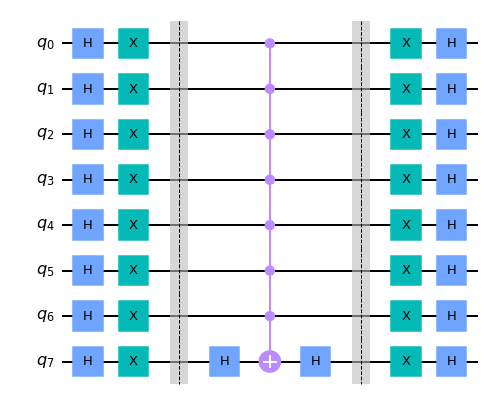
\includegraphics[scale=0.7]{fig05.03.png}
     \caption{The Diffuser for 8 qubits}
     \label{Fig:5.3}
   \end{minipage}
\end{figure}

\subsection{Number of Iterations}
Let our register consist of $n$ qubits. The number of pure states possible is then $2^n=N$. Consider the initial state of the system, where the system is initialized to $\ket{+++\cdots+}$. This is nothing but an equal superposition of the $N$ pure states. Since $\ket{\omega}$ is one of these states and all states occur with equal probabilities, probability of finding $\ket{\omega}$ is $\bfrac{1}{N}=\bfrac{1}{2^n}$. Now, from equation \ref{eq:5.4}, the probability of measuring $\ket{\omega}$ is $\sin^2\theta$. Thus we have,
\begin{equation}
\label{eq:5.8}
\begin{split}
\sin^2\theta&=\bfrac{1}{2^n}\\
\Rightarrow \sin\theta&=\sqrt{\bfrac{1}{2^n}}\\
\end{split}
\end{equation}
At each iteration we reflect by 2$\theta$. Thus, after $k$ iterations, we arrive at angle 2$k\theta$. For complete search, 2$k\theta$ should be as close as possible to $\bfrac{\pi}{2}$ but less than that (to avoid overshoot). For small $theta$, $\sin\theta\approx\theta$. Thus, we have
\begin{equation}
\label{eq:5.9}
\begin{split}
2k\theta&=\bfrac{\pi}{2}\\
\Rightarrow k\sqrt{\bfrac{1}{2^n}}&=\bfrac{\pi}{4}\\
\Rightarrow k&=\bfrac{\pi}{4}\sqrt{2^n}\\
\Rightarrow k&=\bfrac{\pi}{4}\sqrt{N}
\end{split}
\end{equation}
Thus, our complexity of search is $\mathcal{O}(\sqrt{N})$ as compared to $\mathcal{O}(N)$ for a classical brute force method. Further, if there are $M$ solutions instead of one and we are interested in finding at least one solution, the complexity of Grover's algorithm is $\mathcal{O}\left(\sqrt{\bfrac{N}{M}}\right)$.


\subsection{Generalized Grover Search}
Generalized Grover search\cite{gengrov} dwells on the main Grover Search algorithm, except that it reduces the number of gates required by using suitable alternate unitary gates. This further increases the efficiency of the algorithm.\\
The original grover iterate takes the form $G=OAM_0A^\dagger$, where $A$ is any unitary operator (we have used the Hadamard) and $O$ is the oracle. The $M_0$ represents the mirroring circuit. $M_0$ has the form $M_0=X^{\otimes n}M_1X^{\otimes n}$, where $M_1$ is the mirror flip of the last bit implemented using the multi-controlled $Z$-gate. Thus, we have $G=OAM_0A^\dagger=OAX^{\otimes n}M_1X^{\otimes n} A^\dagger$. Setting $B=AX^{\otimes n}$ gives $B^\dagger=X^{\otimes n} A^\dagger$ since $X^{\otimes n\dagger}=X^{\otimes n}$.We can then write $G=OBM_1B^\dagger$, where $M_1$ is a single gate and $B$ avoids the use of $=X^{\otimes n}$, thereby reducing the total number of gates.
\newpage
\section{Our Work}
In this section, we shall present our work. Our work essentially includes designing a suitable hash function and then cracking it using Generalized Grover Search algorithm. The entire code is available at %link to code.
We are working on \textbf{8-bit hashes}. Note that we will use the \textbf{little-endian system} throughout, i.e., $S_0$ represents the Most Significant Bit and $S_7$ the Least Significant Bit.
\subsection{Classical Hashing Algorithm}
The hashing algorithm followed is the 8-bit Pearson Hash generation using 2 LFSRs. The taps for the first LFSR are at indices $3$, $4$, $5$ and $7$. The taps for the second LFSR are at indices $1$, $2$, $4$ and $7$. The diagrams for the same are presented in figures \ref{Fig:6.1} and \ref{Fig:6.2} respectively.
\begin{figure}[!htb]
   \begin{minipage}{\textwidth}
     \centering
     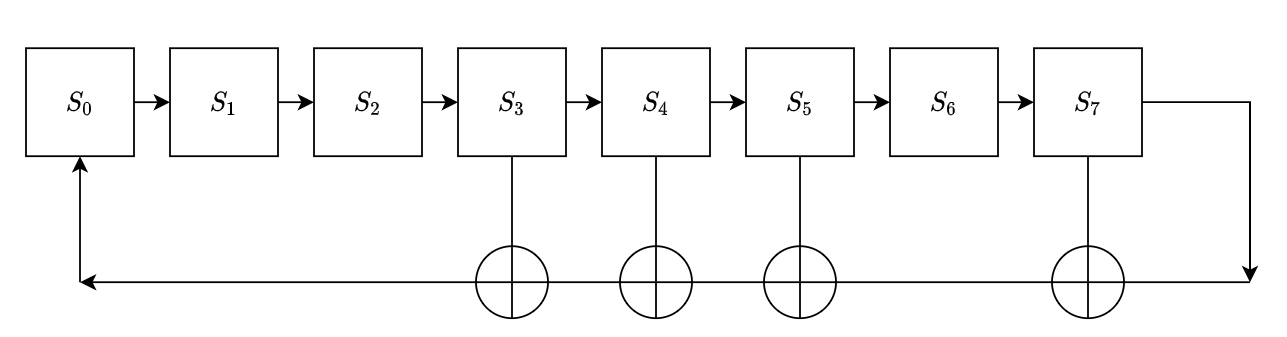
\includegraphics[width=\linewidth]{fig06.01.png}
     \caption{The First LFSR}
     \label{Fig:6.1}
   \end{minipage}
   \begin{minipage}{\textwidth}
     \centering
     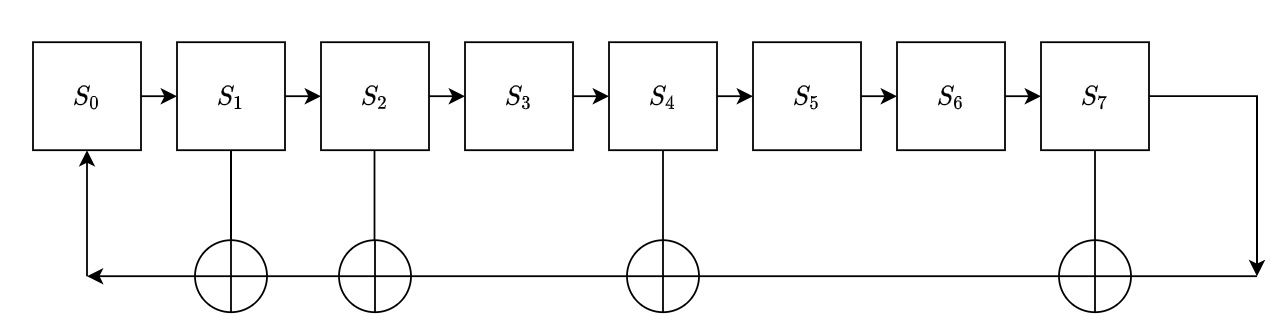
\includegraphics[width=\linewidth]{fig06.02.png}
     \caption{The Second LFSR}
     \label{Fig:6.2}
   \end{minipage}
\end{figure}
Characters are read from the message one at a time. The register is updates by taking its XOR with the ASCII of the character. The new value obtained is then passed through the first LFSR, followed by the second LFSR. The process is repeated for all characters till the end of the message. The code for the same is shown below.
\begin{lstlisting}
def LFSR1_Classical(x):
    bit = ((x >> 0) ^ (x >> 2) ^ (x >> 3) ^ (x >> 4)) & 1
    x = ((x >> 1)|(bit<<7))%256;
    return x
def LFSR2_Classical(x):
    bit = ((x >> 0) ^ (x >> 3) ^ (x >> 5) ^ (x >> 6)) & 1
    x = ((x >> 1)|(bit<<7))%256;
    return x
def hash_Classical(message):
    x=0
    for i in message:
        x=x^ord(i)
        x=LFSR1_Classical(x)
        x=LFSR2_Classical(x)
    return x

message=input().rstrip()
print(hash_Classical(message))
\end{lstlisting}
Now we shall check the values of the hash for some sample strings. This can be done by running the code given above.\\
Message: \verb|Hello World|\\
Hash: \verb|15|\\
Making a slight change\\
Message: \verb|Hello Workd|\\
Hash: \verb|239|\\
We see that the hash changes significantly.

\subsection{Quantum Hashing Algorithm}
Now we will implement the same hashing algorithm on a quantum computer. This will make use of one quantum register comprising $8$ qubits. The nonce itself will be stored on a register of 8 qubits. One qubit will be the output qubit that decides if a given hash is valid or not. Thus, our circuit will make use of $17$ qubits in total, along with some classical bits.  
\subsubsection*{The Two LFSRs and Their Inverses}
Let us first take a look at the two LFSR circuits, given in figures \ref{Fig:6.3} and \ref{Fig:6.4} respectively. These LFSRs perform the same function as the classical LFSRs, except that they do it on qubits.
\begin{figure}[!htb]
   \begin{minipage}{\textwidth}
     \centering
     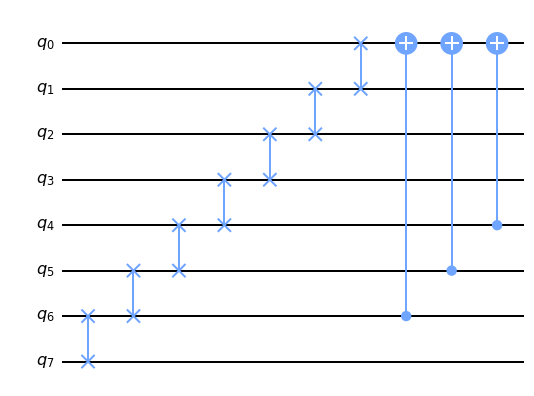
\includegraphics[width=0.9\linewidth]{fig06.03.png}
     \caption{The First LFSR}
     \label{Fig:6.3}
   \end{minipage}
   \begin{minipage}{\textwidth}
     \centering
     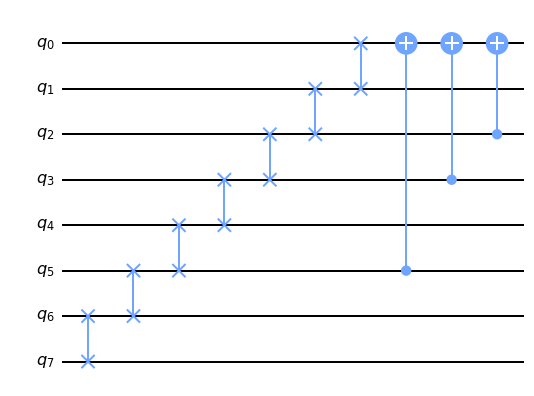
\includegraphics[width=0.9\linewidth]{fig06.04.png}
     \caption{The Second LFSR}
     \label{Fig:6.4}
   \end{minipage}
\end{figure}

For a quantum computer, it is imperative that after each iteration, the registers are restored to the original state for the next iteration to take place successfully. We need to design the circuits for inverting the LFSRs as well. These circuits are shown in figures \ref{Fig:6.5} and \ref{Fig:6.6} respectively.
\begin{figure}[!htb]
   \begin{minipage}{\textwidth}
     \centering
     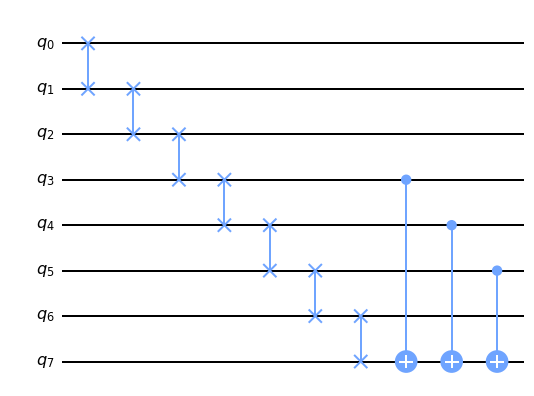
\includegraphics[width=0.9\linewidth]{fig06.05.png}
     \caption{Inverse of the First LFSR}
     \label{Fig:6.5}
   \end{minipage}
   \begin{minipage}{\textwidth}
     \centering
     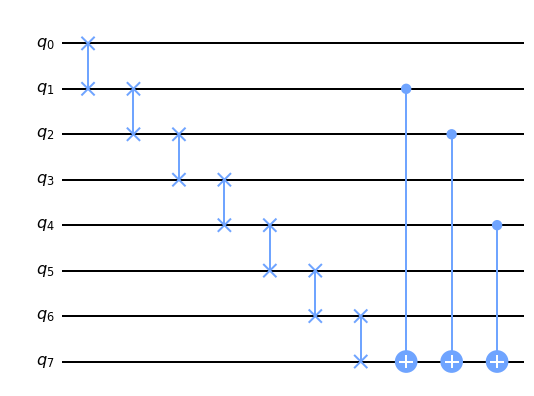
\includegraphics[width=0.9\linewidth]{fig06.06.png}
     \caption{Inverse of the Second LFSR}
     \label{Fig:6.6}
   \end{minipage}
\end{figure}

\subsubsection*{The Hashing Operation}
\noindent The hashing is performed in the following steps.
\begin{enumerate}
\item The classical algorithm is used to compute the hash till the end of the message block, just before the nonce.
\item The quantum hash register of $8$ qubits is initialized with the hash generated.
\item The nonce is XORed with the hash register using CX gates.
\item The first LFSR with taps at $3$, $4$, $5$ and $7$ is operated once on the hash register.
\item The second LFSR with taps at $1$, $2$, $4$ and $7$ is operated once on the hash register.
\end{enumerate}
The circuit for the entire hashing operator is shown in figure \ref{Fig:6.7}.
\begin{figure}[!htb]
   \begin{minipage}{\textwidth}
     \centering
     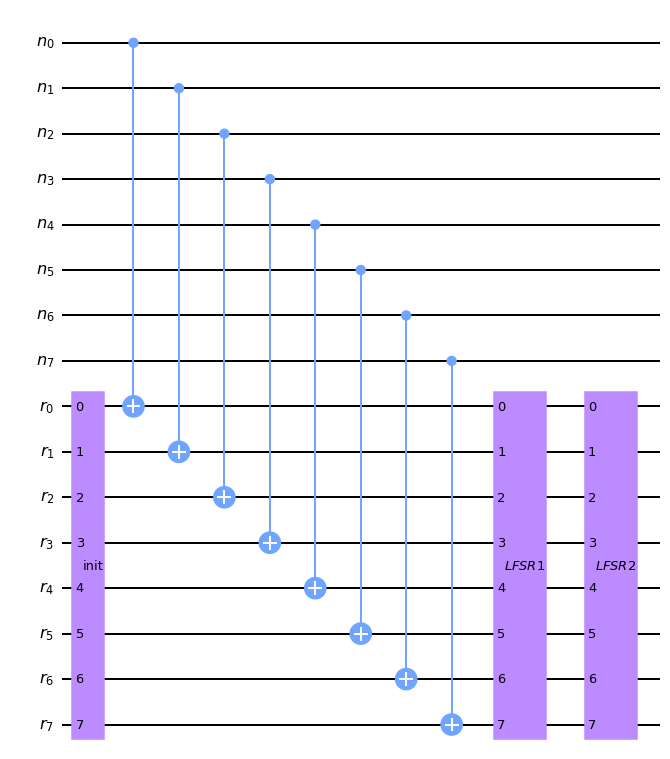
\includegraphics[width=0.8\linewidth]{fig06.07.png}
     \caption{Hashing Circuit}
     \label{Fig:6.7}
   \end{minipage}
\end{figure}

\subsubsection*{The Oracle}
It is now time to put everything together. We shall assume that a valid nonce is one that starts with $5$ zeroes. For this, we need to check if the registers at indices $0$, $1$, $2$, $3$ and $4$ are $\ket{0}$. A multi-controlled Toffoli gate from these register qubits to the output will flip the qubits of the output if and only if all of the $5$ qubits were $\ket{1}$. Further, if the output is initialized to $\ket{out}=\bfrac{\ket{0}-\ket{1}}{\sqrt{2}}$, we will get the output to flip sign only when all of the $5$ qubits are $\ket{1}$ or else output stays the same. Since we are interested in checking if all the $5$ qubits are $\ket{0}$, we must use $X$ gates on them before passing them through the multi-controlled Toffoli gate. After the check, we must restore the registers by inverting the operations applied. This invovles taking an $X$ gate on qubits $0$, $1$, $2$, $3$ and $4$, followed by the inverse of the second LFSR, followed by the inverse of the first LFSR. Figure \ref{Fig:6.8} shows the complete oracle circuit.
\begin{figure}[!htb]
   \begin{minipage}{\textwidth}
     \centering
     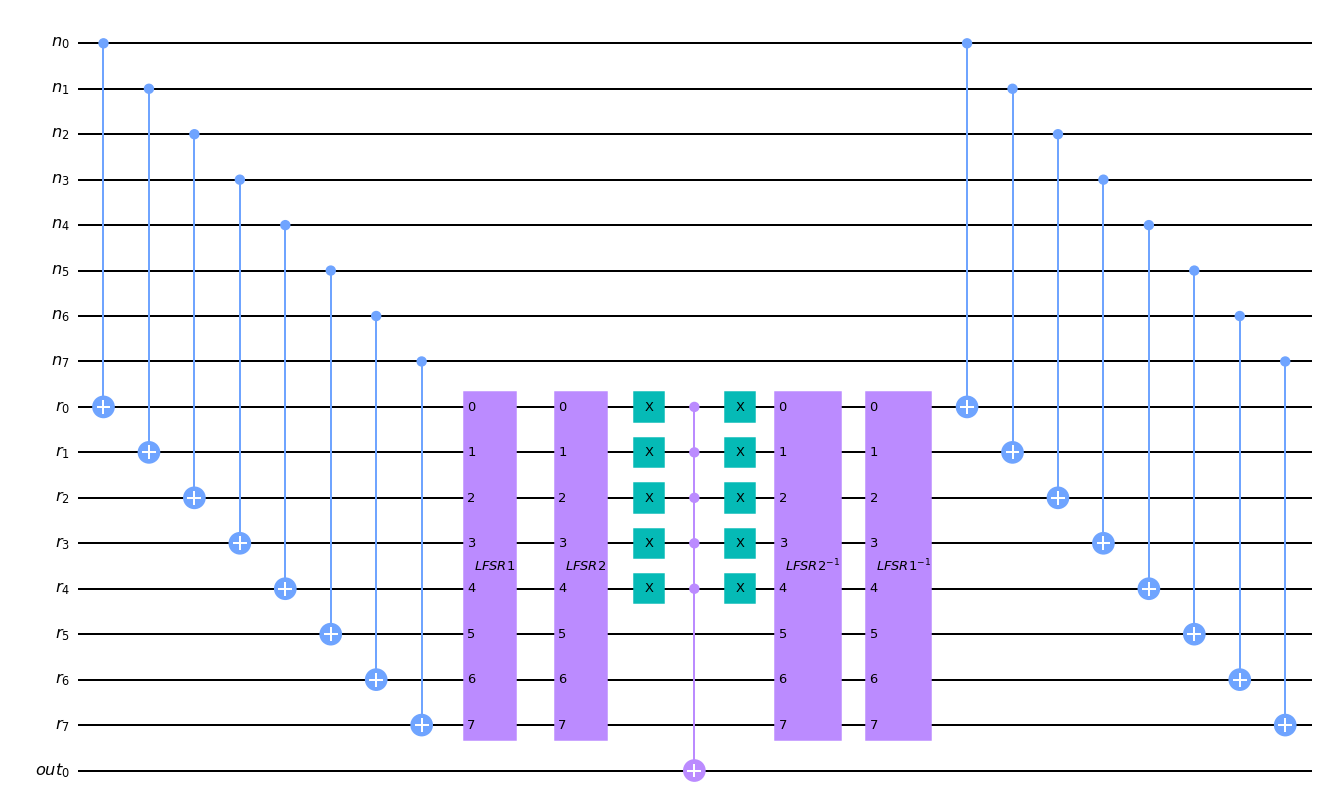
\includegraphics[width=\linewidth]{fig06.08.png}
     \caption{Circuit for the Oracle}
     \label{Fig:6.8}
   \end{minipage}
\end{figure}

\subsubsection*{Grover Search}
The grover search involves setting up the nonce to a superposition of all states using a $H$ gate on all the qubits followed by the repeated application of the oracle followed by the diffuser. The diffuser used has been discussed in the section preceding figure \ref{Fig:5.3}. The number of iterations required is given by equation \ref{eq:5.9}, where, we now have $M=8$ solutions instead of $1$. Thus, number of iterations, $k$, is
\begin{equation}
\label{eq:6.1}
k=\left\lfloor\bfrac{\pi}{4}\sqrt{\bfrac{N}{M}}\right\rfloor=\left\lfloor\bfrac{\pi}{4}\sqrt{\bfrac{256}{8}}\right\rfloor=4
\end{equation}
Finally, we perform a measurement of the nonce. Figure \ref{Fig:6.9} shows the entire circuit.
\begin{figure}[!htb]
   \begin{minipage}{\textwidth}
     \centering
     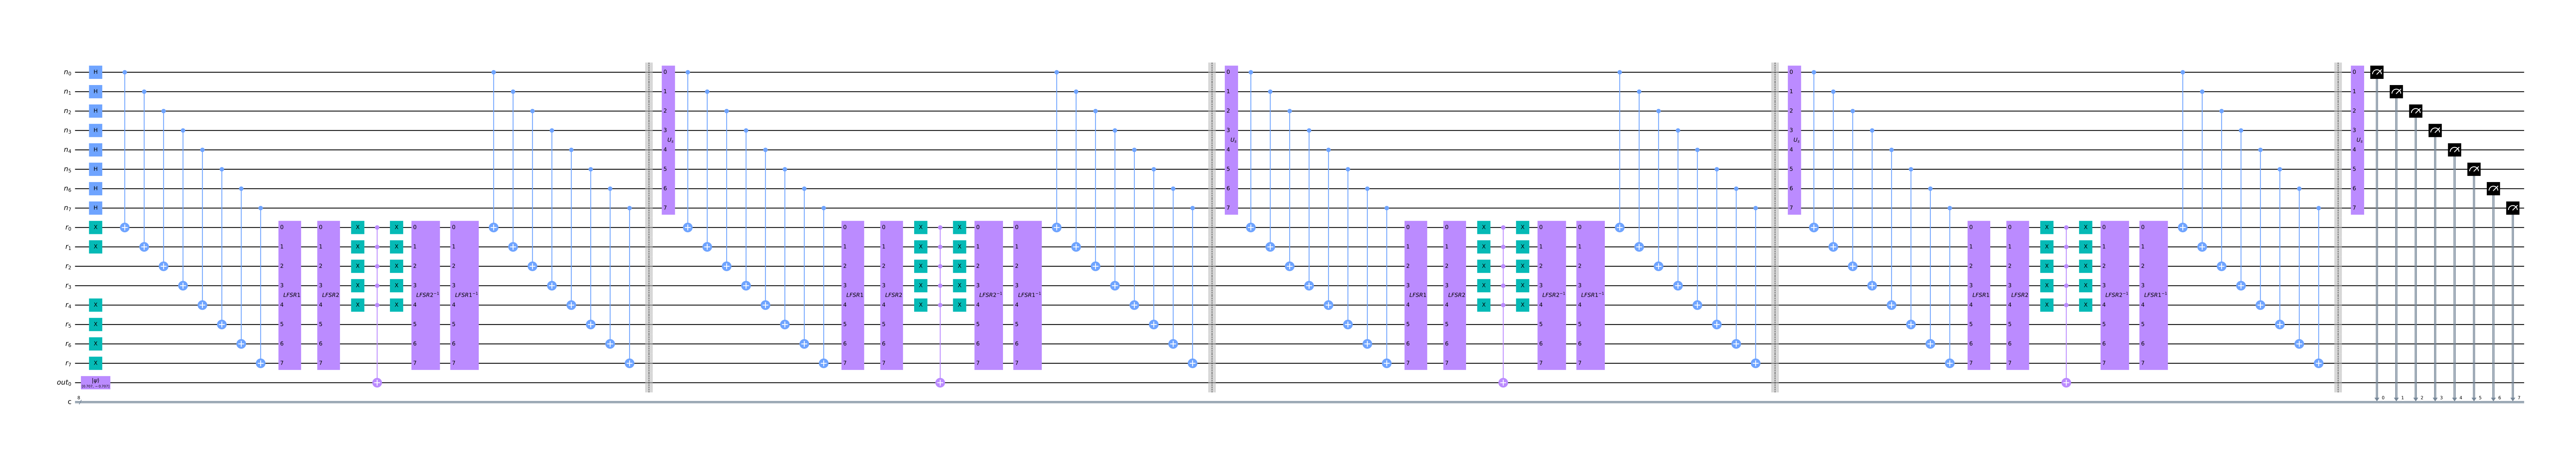
\includegraphics[width=\linewidth]{fig06.09.png}
     \caption{Grover Search Circuit}
     \label{Fig:6.9}
   \end{minipage}
\end{figure}

\subsubsection*{Generalized Grover Search}
Here, we replace the $H$ gate followed by $X$ gate by a single unitary gate. $R_y\left(\bfrac{\pi}{2}\right)$ is a suitable unitary transformation substitute for $HX$. Its inverse is $R_y\left(-\bfrac{\pi}{2}\right)$. We can then simplify our diffuser to the one given in figure \ref{Fig:6.10} thereby reducing 16 gates per iteration.
\begin{figure}[!htb]
   \begin{minipage}{\textwidth}
     \centering
     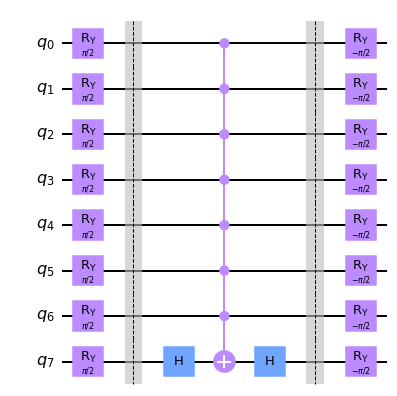
\includegraphics[scale=0.6]{fig06.10.png}
     \caption{Generalised Grover Diffuser}
     \label{Fig:6.10}
   \end{minipage}
\end{figure}
This reduction in the number of gates is very helpful. We will do an analysis of the same in the next section.


\newpage
\section{Results}
In this section, we shall see the results obtained after performing the Grover Search. Since we are using the \textbf{little-endian} system, the output qubits obtained must be read from right to left to get the ASCII value of the nonce-character. We will then append the nonce to the message and check if its classical hash indeed starts with $5$ zeroes when written in binary.

\subsubsection*{Number of Gates}
\noindent First we observe the difference in the number of gates used in the Grover and the Generalized Grover Search algorithms. To count the gates, we split them as follows\\

\noindent Each LFSR (or LFSR inverse) has\\
7 $SWAP$ gates\\
3 $CX$ gates\\

\noindent Each Diffuser has\\
18 $H$ gates\\
16 $X$ gates\\
1 $MCT$ gate\\

\noindent Each Generalized Diffuser has\\
16 $R_y$ gates\\
2 $H$ gates\\
1 $MCT$ gate\\

\noindent Each iteration has\\
2 LFSRs\\
2 Inverse LFSRs\\
1 Diffuser (or Generalized Diffuser)\\
16 $CX$ gates\\
10 $X$ gates\\
1 $MCT$ gate\\

There are 8 $H$ gates at the start followed by 4 iterations. Thus the total number of gates can be summarized by table \ref{Tab:7.1}.

\begin{table}[!htb]
\centering
	\begin{tabular}{|M{5cm}|M{1.5cm}|M{1.5cm}|M{1.5cm}|M{1.5cm}|M{1.5cm}|M{1.5cm}|M{2cm}|}
		\hline
		\multicolumn{8}{|c|}{\addmathvspace\textbf{SUMMARY OF THE NUMBER OF GATES USED}}\\
		\hline
		\addmathvspace\textbf{Algorithm} & 
		$\mathbf{H}$ &
		$\mathbf{X}$ &
		$\mathbf{CX}$ &
		$\mathbf{SWAP}$ &
		$\mathbf{MCT}$ & 
		$\mathbf{R_y}$ & 
		$\mathbf{TOTAL}$\\[5pt]
		\hline
		Grover Search&80&104&112&112&8&0&416\\[3pt]
		\hline
		Generalized Grover Search&16&40&112&112&8&64&352\\[3pt]
		\hline		
	\end{tabular}
	\caption{Table summarizing the number of gates required}
	\label{Tab:7.1}
\end{table}
\FloatBarrier
We observe that the Generalized Grover Search algorithm uses significantly less number of gates.

\subsubsection*{Qiskit Simulation}
\noindent Here, we will use the \textbf{aer\_simulator} provided by qiskit to run our code.
For testing purposes our message is\\
Message: \verb|Hello World|\\
This is then passed on to our program. A simulation of 1024 measurements is done. The result is shown in figure \ref{Fig:7.1}.
\begin{figure}[!htb]
   \begin{minipage}{\textwidth}
     \centering
     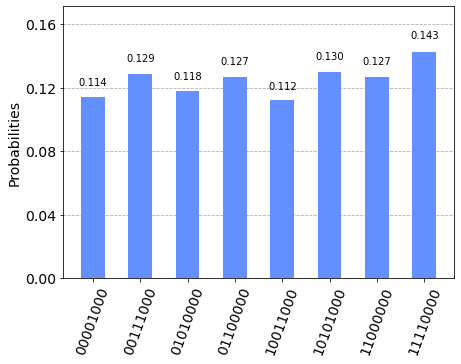
\includegraphics[scale=0.8]{fig07.01.png}
     \caption{Nonce values obtained and their probabilities}
     \label{Fig:7.1}
   \end{minipage}
\end{figure}
Note that since all since we are using the \textbf{little-endian} system, output must be read from right to left. Converting the binary to decimal, we get the ASCII of the nonce to be appended as \\

\begin{minipage}{\textwidth}
\begin{lstlisting}
28
3
21
25
15
6
10
16
\end{lstlisting}
\end{minipage}

We append the nonce and test the output hashes. The output hashes are (in the same order as the nonce values)\\

\begin{minipage}{\textwidth}
\begin{lstlisting}
4
3
6
5
0
2
1
7
\end{lstlisting}
\end{minipage}

Thus, we conclude that our algorithm works successfully.

\newpage
\section{Future Work to be Done}
This section highlights the work left to be done in the subsequent interactions.
\subsection{Testing on Real Quantum Hardware}
So far all the results obtained are the outputs of simulations of the quantum circuits on a classical computer. The next phase will deal with actually using an IBM quantum system to execute the circuit. The circuit is quite heavy (17 qubits) and requires significant amount of quantum computing resources to execute. We will figure this out and check the probability distributions from a real quantum computer\cite{qsys}. 
\subsection{Developing a Secure Blockchain Using Entanglement}
We will use the Bell's Measure and the CSHS inequality to develop a secure blockchain\cite{ent}\cite{qkd}.
\subsection{Quantum Hashing}
We will develop some novel hashing algorithms that are purely quantum mechanical and cannot be implemented on a classical computer.
\newpage
\bibliography{refs}

\end{document}

